\documentclass[11pt]{article}
\usepackage[toc,page]{appendix}
\usepackage{amsmath, amssymb}
\usepackage[utf8]{inputenc}
\usepackage[T1]{fontenc}
\usepackage[style=apa,backend=biber]{biblatex}
%\usepackage{biblatex}
\addbibresource{references.bib}
\usepackage{graphicx}
\usepackage{tikz}
\usetikzlibrary{automata,positioning,shapes.geometric, arrows.meta, fit, backgrounds, calc, chains}
\graphicspath{./images/Easy_Pictures/SMR_MULT_Repackaging}%\usepackage{kpfonts}
\usepackage{float}
\usepackage[margin=1in]{geometry}
\usepackage{cancel}
\usepackage{epsfig}
\usepackage{enumitem}
\usepackage{tikz-3dplot}
\usepackage{darkmode}
\usepackage{dirtytalk}
\usepackage{longtable,booktabs,array}
\usepackage{calc} % for calculating minipage widths
\usepackage[utf8]{inputenc}
\usepackage[T1]{fontenc}
\usepackage{xcolor}
\usepackage{listings}


\usepackage{etoolbox}
\usepackage{hyperref}
\hypersetup{
    colorlinks=true,
    linkcolor=blue,
    filecolor=magenta,      
    urlcolor=cyan,
    pdftitle={Hermeneutic Calculator},
    citecolor=blue,
    }


\urlstyle{same}

\lstdefinestyle{htmlStyle}{
    language=HTML,
    basicstyle=\ttfamily\small,
    keywordstyle=\color{blue}\bfseries,
    commentstyle=\color{gray}\itshape,
    stringstyle=\color{red},
    breaklines=true,
    frame=single,
    numbers=left,
    numberstyle=\tiny\color{gray},
    columns=fullflexible,
}
\lstdefinelanguage{HTML}{
  keywords={<!DOCTYPE, html, head, title, body, h1, h2, h3, p, div, span, a, img, ul, li, table, tr, td, th, style, link, script},
  sensitive=true,
  comment=[l]{//},
  morecomment=[s]{/*}{*/},
  morestring=[b]',
  morestring=[b]"
}
\lstset{style=htmlstyle, language=html}
% Updated to explicitly pass the language option
%\lstinputlisting[style=htmlstyle, language=html]{./html/example.html}
%\usepackage{tocloft}

% Optional: define some custom colors
\definecolor{sliceRed}{RGB}{225,224,91} % matching "varyellow" from your code
\definecolor{linkYellow}{RGB}{255,215,0}  % a golden yellow
\tdplotsetmaincoords{70}{110}

\title{Subtraction Strategies: Chunking}
\author{Compiled by: Theodore M. Savich}


\begin{document}
\maketitle



\subsection*{Transcript}
Video from \textcite{Carpenter1999}. Strategy descriptions and examples adapted from \textcite{HackenbergCourseNotes}. 


\begin{itemize}
    \item \textbf{Teacher:}``One summer T.J. saved \$400. At the end of the summer she spent \$294 on a new bike. How much money did T.J. have then?''
    \item \textbf{Student:} ``400 takeaway 200 is 200. I just put the 4 on the side right now. So then 200 takeaway 90 is 110. So then 110 takeaway 4 is 106. 
    \item \textbf{Teacher:} ``So how much money did she have left?''
    \item \textbf{Student:} ``106.''
    \item \textbf{Teacher:} ``Nice job.''
\end{itemize}

Here is the notation below to show what the student did:

\begin{align*}
400 - 200 &= 200\\
200 - 90 &= 110\\
110 - 4 &= 106
\end{align*}


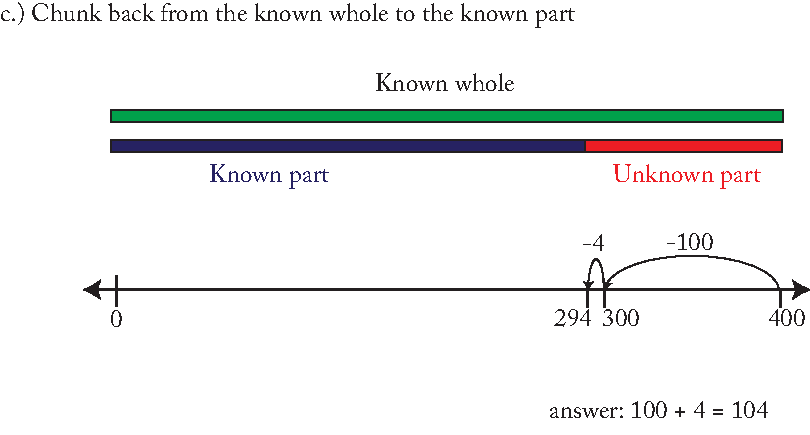
\includegraphics[width=.8\textwidth]{images/Easy_Pictures/SAR_SUB_CHUNKING_3_Ways/PDF/CHUNKING_BACKWARD_TO_KNOWN_PART.pdf}


However, this is only one of three structurally different ways that chunking can show up in subtraction. 

\begin{enumerate}[label=(\alph*)]
    \item \textbf{Chunking backwards (by known part)} The student starts at the known whole and subtracts backwards by the known part. They arrive at the unknown part. 
    \item \textbf{Chunking forwards} The student subtracts the known whole from the known part. 
    \item \textbf{Chunking backwards (to the known part)}  The student starts at the known whole and subtracts backwards until they reach the known part.
\end{enumerate}



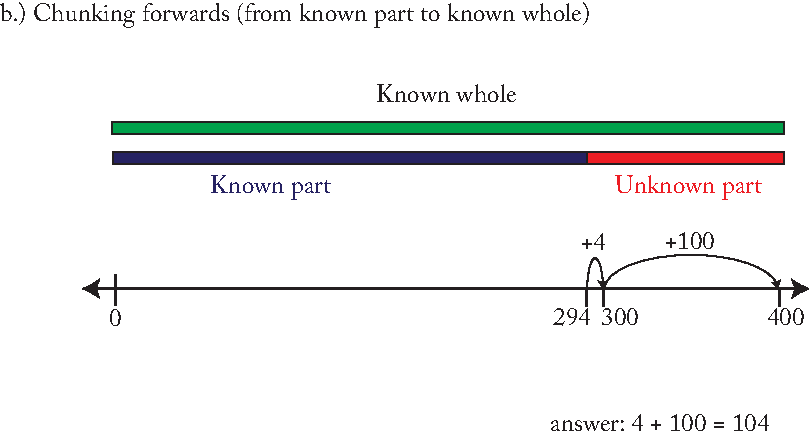
\includegraphics[width=.8\textwidth]{images/Easy_Pictures/SAR_SUB_CHUNKING_3_Ways/PDF/CHUNKING_FORWARD_FROM_KNOWN_PART.pdf}


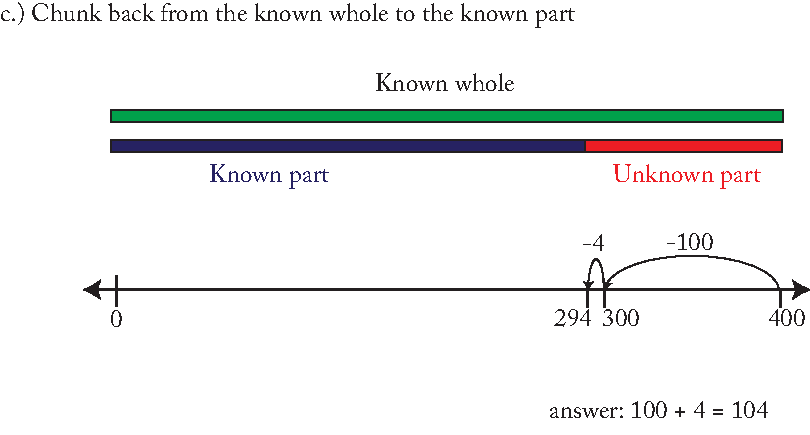
\includegraphics[width=.8\textwidth]{images/Easy_Pictures/SAR_SUB_CHUNKING_3_Ways/PDF/CHUNKING_BACKWARD_TO_KNOWN_PART.pdf}


\subsubsection*{Description of Strategy}
\begin{itemize}
    \item Subtract the subtrahend (known part) from the minuend (known whole) by breaking the subtrahend into bases and ones and subtracting in strategic chunks. 
    \item Start from the subtrahend and add strategic chunks to reach the minuend, summing the chunks to find the difference.
    \item Start at the minuend and subtract strategic chunks until you reach the subtrahend, summing the chunks to find the difference.
\end{itemize}

\subsubsection*{Corrected Automaton (Register Machine) and Python Implementation}

We implement corrected Register Machines for all three strategies. Strategies B and C explicitly include iterative subroutines (based on RMB logic) to model the cognitive process of determining strategic chunks.

\begin{lstlisting}[language=Python]
import pandas as pd
import math

class SubtractionChunkingAutomaton:
    """Base class for subtraction chunking strategies."""
    def __init__(self, M, S, Base=10):
        self.M = M # Minuend (Whole)
        self.S = S # Subtrahend (Known Part)
        self.Base = Base
        self.history = []
        self.state = 'q_start'
        self.Result = 0

        if S > M:
            self.state = 'q_error'
            self._record_history(f"Error: Subtrahend ({S}) > Minuend ({M}).")

    def _record_history(self, interpretation, **kwargs):
        record = {'State': self.state, 'Interpretation': interpretation}
        record.update(kwargs)
        self.history.append(record)

    def transition(self, next_state):
        self.state = next_state

    def run(self):
        while self.state not in ['q_accept', 'q_error']:
            # Dynamically call the method corresponding to the state
            executor = getattr(self, f"execute_{self.state}", self.execute_error)
            executor()
        return self.Result

    def execute_error(self):
        if self.state != 'q_error':
            self._record_history(f"Error: Entered unknown state {self.state}")
            self.transition('q_error')

    def display_history(self):
        print(f"\n--- Subtraction Chunking History ({self.M} - {self.S}) | Strategy: {self.strategy_name} ---")
        df = pd.DataFrame(self.history)
        if not df.empty:
            df = df.fillna('')
        print(df.to_markdown(index=False))

# =============================================================================
# Strategy A: Chunking Backwards (by Known Part) - Place Value Decomposition
# =============================================================================

class ChunkingAutomatonA(SubtractionChunkingAutomaton):
    """
    Strategy A: Start at M, subtract chunks of S decomposed by place value.
    """
    strategy_name = "A (Backwards by Part)"
    
    def __init__(self, M, S, Base=10):
        super().__init__(M, S, Base)
        self.CurrentValue = 0
        self.S_Remaining = 0

    def execute_q_start(self):
        self._record_history("Start: Initialize.", CV=0, S_Rem=0)
        self.transition('q_init')

    def execute_q_init(self):
        self.CurrentValue = self.M
        self.S_Remaining = self.S
        self._record_history(f"Set CurrentValue={self.M}. S_Remaining={self.S}.", CV=self.CurrentValue, S_Rem=self.S_Remaining)
        self.transition('q_identify_chunk')

    def execute_q_identify_chunk(self):
        """Identify the next chunk of S by largest place value."""
        if self.S_Remaining == 0:
            self.Result = self.CurrentValue
            self._record_history(f"S fully subtracted. Result={self.Result}.", CV=self.CurrentValue, S_Rem=0)
            self.transition('q_accept')
            return

        # Identify the largest place value chunk remaining in S_Remaining
        # Generalized approach using log to handle any base
        if self.S_Remaining > 0:
            power = math.floor(math.log(self.S_Remaining, self.Base))
            power_value = self.Base**power
            # Calculate the chunk (e.g., the '200' in 294)
            Chunk = (self.S_Remaining // power_value) * power_value
        else:
            Chunk = 0

        self.Chunk = Chunk
        self._record_history(f"Identified chunk to subtract: {Chunk}.", CV=self.CurrentValue, S_Rem=self.S_Remaining)
        self.transition('q_subtract_chunk')

    def execute_q_subtract_chunk(self):
        """Subtract the identified chunk."""
        Chunk = self.Chunk
        self.CurrentValue -= Chunk
        self.S_Remaining -= Chunk
        self._record_history(f"Subtracted {Chunk}. New Value={self.CurrentValue}.", CV=self.CurrentValue, S_Rem=self.S_Remaining)
        self.transition('q_identify_chunk') # Loop back

# =============================================================================
# Strategy B: Chunking Forwards (Missing Addend) - RMB Logic
# =============================================================================

class ChunkingAutomatonB(SubtractionChunkingAutomaton):
    """
    Strategy B: Start at S, add up to M. Result is the distance traveled.
    Uses strategic addition (RMB logic) modeled iteratively.
    """
    strategy_name = "B (Forwards from Part)"

    def __init__(self, M, S, Base=10):
        super().__init__(M, S, Base)
        self.CurrentValue = 0
        self.Distance = 0
        # Internal registers for iterative K calculation (RMB subroutine)
        self.K = 0
        self.TargetBase = 0
        self.internal_temp = 0

    def transition(self, next_state):
        # Reset K/RMB registers when exiting the RMB loop
        if next_state == 'q_check_status':
             self.K = 0
             self.TargetBase = 0
             self.internal_temp = 0
        self.state = next_state

    def execute_q_start(self):
        self._record_history("Start: Initialize.", CV=0, Dist=0)
        self.transition('q_init')

    def execute_q_init(self):
        self.CurrentValue = self.S
        self.Distance = 0
        self._record_history(f"Start at S ({self.S}). Target is M ({self.M}).", CV=self.CurrentValue, Dist=self.Distance)
        self.transition('q_check_status')

    def execute_q_check_status(self):
        if self.CurrentValue < self.M:
            self.transition('q_init_K')
        else:
            self.Result = self.Distance
            self._record_history(f"Target reached. Result (Distance)={self.Result}.", CV=self.CurrentValue, Dist=self.Distance)
            self.transition('q_accept')

    # RMB Subroutine (Iterative Count Up To Base)
    def execute_q_init_K(self):
        """Initialize iterative calculation of K to reach the next strategic base."""
        self.K = 0
        self.internal_temp = self.CurrentValue

        # Determine the next target base (Prioritizing lower powers of the base)
        # Example in Base 10: Prioritize 10s, then 100s, etc.
        self.TargetBase = self.CurrentValue
        power = 1
        while True:
            BasePower = self.Base**power
            if self.CurrentValue % BasePower != 0:
                self.TargetBase = ((self.CurrentValue // BasePower) + 1) * BasePower
                break
            # If we exceed the target M, we stop prioritizing boundaries.
            if BasePower > self.M:
                break
            power += 1

        self._record_history(f"Calculating K: Counting from {self.CurrentValue} to {self.TargetBase}.", CV=self.CurrentValue, Dist=self.Distance, K=0)
        self.transition('q_loop_K')

    def execute_q_loop_K(self):
        if self.internal_temp < self.TargetBase:
            # Iterative step (Counting Up)
            self.internal_temp += 1
            self.K += 1
        else:
            self.transition('q_add_chunk')

    def execute_q_add_chunk(self):
        """Determine the chunk to add based on K or remaining distance."""
        Remaining = self.M - self.CurrentValue

        # Strategy 1: Use K if it's useful (K>0) and doesn't overshoot
        if self.K > 0 and self.K <= Remaining:
            Chunk = self.K
            Interpretation = f"Add strategic chunk (+{Chunk}) to reach base."
        # Strategy 2: If K is 0 (already at a base), add largest multiple of power of base possible.
        else:
            if Remaining > 0:
                power = math.floor(math.log(Remaining, self.Base))
                power_value = self.Base**power
                Chunk = (Remaining // power_value) * power_value
                Chunk = Chunk if Chunk > 0 else Remaining
                Interpretation = f"Add large/remaining chunk (+{Chunk})."
            else:
                self.transition('q_error'); return

        self.CurrentValue += Chunk
        self.Distance += Chunk
        self._record_history(Interpretation + f" New Value={self.CurrentValue}.", CV=self.CurrentValue, Dist=self.Distance, K=self.K)
        self.transition('q_check_status')

# =============================================================================
# Strategy C: Chunking Backwards (to Known Part) - Inverse RMB Logic
# =============================================================================

class ChunkingAutomatonC(SubtractionChunkingAutomaton):
    """
    Strategy C: Start at M, subtract down to S. Result is the distance traveled.
    Uses strategic subtraction (Reverse RMB logic) modeled iteratively.
    """
    strategy_name = "C (Backwards to Part)"

    # Initialization and structure mirror Strategy B, but direction is reversed.
    def __init__(self, M, S, Base=10):
        super().__init__(M, S, Base)
        self.CurrentValue = 0
        self.Distance = 0
        self.K = 0
        self.TargetBase = 0
        self.internal_temp = 0

    def transition(self, next_state):
        if next_state == 'q_check_status':
             self.K = 0
             self.TargetBase = 0
             self.internal_temp = 0
        self.state = next_state

    def execute_q_start(self):
        self._record_history("Start: Initialize.", CV=0, Dist=0)
        self.transition('q_init')

    def execute_q_init(self):
        self.CurrentValue = self.M # Start at M
        self.Distance = 0
        self._record_history(f"Start at M ({self.M}). Target is S ({self.S}).", CV=self.CurrentValue, Dist=self.Distance)
        self.transition('q_check_status')

    def execute_q_check_status(self):
        if self.CurrentValue > self.S: # Loop until S is reached
            self.transition('q_init_K')
        else:
            self.Result = self.Distance
            self._record_history(f"Target reached. Result (Distance)={self.Result}.", CV=self.CurrentValue, Dist=self.Distance)
            self.transition('q_accept')

    # Reverse RMB Subroutine (Iterative Count Back To Base)
    def execute_q_init_K(self):
        """Initialize iterative calculation of K to reach the previous base."""
        self.K = 0
        self.internal_temp = self.CurrentValue

        # Determine the previous target base
        self.TargetBase = self.CurrentValue
        power = 1
        while True:
            BasePower = self.Base**power
            if self.CurrentValue % BasePower != 0:
                self.TargetBase = (self.CurrentValue // BasePower) * BasePower
                break
            # If we go below the target S, we stop prioritizing boundaries.
            if BasePower > self.M:
                 break
            power += 1

        self._record_history(f"Calculating K: Counting back from {self.CurrentValue} to {self.TargetBase}.", CV=self.CurrentValue, Dist=self.Distance, K=0)
        self.transition('q_loop_K')

    def execute_q_loop_K(self):
        if self.internal_temp > self.TargetBase:
            # Iterative step (Counting Back)
            self.internal_temp -= 1
            self.K += 1
        else:
            self.transition('q_sub_chunk')

    def execute_q_sub_chunk(self):
        """Determine the chunk to subtract based on K or remaining distance."""
        Remaining = self.CurrentValue - self.S

        # Strategy 1: Use K if it's useful (K>0) and doesn't overshoot
        if self.K > 0 and self.K <= Remaining:
            Chunk = self.K
            Interpretation = f"Subtract strategic chunk (-{Chunk}) to reach base."
        # Strategy 2: If K is 0, subtract largest multiple of power of base possible.
        else:
            if Remaining > 0:
                power = math.floor(math.log(Remaining, self.Base))
                power_value = self.Base**power
                Chunk = (Remaining // power_value) * power_value
                Chunk = Chunk if Chunk > 0 else Remaining
                Interpretation = f"Subtract large/remaining chunk (-{Chunk})."
            else:
                self.transition('q_error'); return

        self.CurrentValue -= Chunk
        self.Distance += Chunk
        self._record_history(Interpretation + f" New Value={self.CurrentValue}.", CV=self.CurrentValue, Dist=self.Distance, K=self.K)
        self.transition('q_check_status')

# =============================================================================
# Testing and Efficiency Analysis
# =============================================================================

# Test Case 1: 400 - 294 (As in the PDF)
M_test = 400
S_test = 294
print(f"=== Test Case: {M_test} - {S_test} ===")

# Test Strategy A
auto_A = ChunkingAutomatonA(M=M_test, S=S_test)
auto_A.run()
auto_A.display_history()

# Test Strategy B
auto_B = ChunkingAutomatonB(M=M_test, S=S_test)
auto_B.run()
auto_B.display_history()

# Test Strategy C
auto_C = ChunkingAutomatonC(M=M_test, S=S_test)
auto_C.run()
auto_C.display_history()

# Test Case 2: 83 - 17 (Efficiency Comparison)
M_test_2 = 83
S_test_2 = 17
print(f"\n=== Efficiency Comparison: {M_test_2} - {S_test_2} ===")

auto_A_2 = ChunkingAutomatonA(M_test_2, S_test_2)
auto_A_2.run()
auto_A_2.display_history()

auto_B_2 = ChunkingAutomatonB(M_test_2, S_test_2)
auto_B_2.run()
auto_B_2.display_history()

auto_C_2 = ChunkingAutomatonC(M_test_2, S_test_2)
auto_C_2.run()
auto_C_2.display_history()
\end{lstlisting}

\printbibliography
\end{document}